\documentclass[a4paper]{article}
\usepackage{graphicx}
\usepackage{subcaption}
\usepackage{amsmath}
\usepackage{amssymb}
\usepackage[utf8]{inputenc}
\usepackage[english]{babel}
\usepackage[
backend=bibtex,
sorting=ynt
]{biblatex}
\addbibresource{bibliography.bib}

\author{Mattia Lecchi (33362A)}
\title{Branch and bound algorithm for SCP with conflict sets\\ 
	\large Project of Operations Research Complements (A.Y. 2024/2025)}

\begin{document}
	\maketitle
	
\section{Introduction}

The project tackle a variant of the Set Covering Problem (SCP) introducing penalties if certain couples of sets are selected. Formally, let $E=\{1,...,n\}$ be a set of elements and let $\mathcal S=\{S_j\subseteq E : j \in M\}$ be the set of subsets, where $M=\{1,...,m\}$. 
The subsets composition is defined by a matrix $A \in \mathbb R^{n\times m}$:
$$
A_{ij} =
\begin{cases}
	1& \text{if } E_i \in S_j\\
	0& \text{otherwise}\\
\end{cases}
$$
The vector $c \in \mathbb R^{m}$ defines the costs for each subset, while the matrix $P \in \mathbb R^{m\times m}$ defines the penalties for each couple of subsets, i.e. $P_{ij}$ is the penalty paid if $S_i,S_j\in \mathcal S$ are both selected.
The IP formulation for the SCP with conflict sets is the following:
\begin{align*}
	\min_{x,y} & \sum_{i\in M} c_i x_i + \sum_{i \in M} \sum_{j \in M} P_{ij} y_{ij} & \\
	\text{s.t. } 
	& \sum_{i\in M} A_{ik} x_i \ge 1 & \forall k \in E \\
	& x_i + x_j \le 1 + y_{ij} & \forall i,j \in M \\
	& x_i \in \{0, 1\} & \forall i \in M \\
	& y_{ij} \in \{0, 1\} & \forall i,j \in M\\
\end{align*}
although it can be noticed that integrality constraints on $y_{ij}$ variables are redundant.
The chosen exact optimization approach is a branch and bound algorithm with Lagrangean relaxation for dual bound computation.

\section{Lagrangean relaxation}

We chose to relax the covering constraints, obtaining the following Lagrangean relaxation:

\begin{align*}
	\min_{x,y} & \sum_{i\in M} c_i x_i + \sum_{i \in M} \sum_{j \in M} P_{ij} y_{ij} + \sum_{k \in E}\sum_{i\in M} \left(\lambda_k A_{ik} x_i - 1\right)  & \\
	\text{s.t. }
	& x_i + x_j \le 1 + y_{ij} & \forall i,j \in M \\
	& x_i \in \{0, 1\} & \forall i \in M \\
	& y_{ij} \in \{0, 1\} & \forall i,j \in M\\
\end{align*}
rewriting the objective function as:
$$
\min_{x,y} \sum_{i\in M} \left(c_i + \sum_{k \in E} \lambda_k A_{ik}\right) x_i + \sum_{i \in M} \sum_{j \in M} P_{ij} y_{ij} - \sum_{k \in E} \lambda_k
$$
we obtain a linear formulation of the quadratic knapsack problem for the Lagrangean primal, plus a constant term. The quadratic knapsack problem is still a NP-hard problem.

\section{Algorithm}

The algorithm is a branch-and-bound using a Lagrangean relaxation for the dual computation on nodes. At each iteration, the algorithm generate 6 children subproblems by fixing the first free choice variables as follows:
\begin{align*}
&x_1 = 1\\
&x_1 = 0, x_2 = 1\\
&x_1 = 0, x_2 = 0, x_3 = 1\\
&x_1 = 0, x_2 = 0, x_3 = 0, x_4 = 1\\
&x_1 = 0, x_2 = 0, x_3 = 0, x_4 = 0, x_5 = 1\\
&x_1 = 0, x_2 = 0, x_3 = 0, x_4 = 0, x_5 = 0.
\end{align*}
The dual bounds for each generated subproblem are computed in parallel, thus the choice of the number of children should be based on the number of CPU cores available. 

Solving the Lagrangean relaxation yields a possibly infeasible solution, that is a subset selection that only partially covers the elements. With a simple greedy repair heuristic, the algorithm compute a primal bound from the dual solution; if the procedure fails to provide a feasible solution considering the currently fixed variables, then the subproblem can be discarded, as none of the next subproblems can reach a feasible solution. Another case in which the next subproblems can be discarded is when the optimal dual of the Lagrangean relaxation yields an optimal solution for the original subproblem, that is when the complementary slackness condition is satisfied:
$$
Ax^* \ge 1 \wedge \lambda^{*T} (1 - Ax^*) = 0
$$
Considering the optimal solution $\lambda^*, x^*$ for the relaxation. The nodes are explored using a depth-first strategy, implemented with a stack. The subproblems generated are pushed in the stack in descending order of dual bound. This ensures that subproblems with lower dual bounds are solved first among siblings.

\subsection{Greedy heuristic}
A simple greedy heuristic is applied on each subproblem to repair the potentially infeasible solution from the Lagrangean relaxation. The algorithm relies on a minimum priority queue, assigning a cost to each subset. The algorithm iteratively extract a subset from the queue until it reaches a feasible solution. The initial costs for a subset $S_i$ is computed as $\hat c_i^{(0)} = c_i/|S_i|$ and is updated at each iteration considering the penalties. Suppose that at iteration $\tau$ the subset $S_j$ is selected; the penalties are updated as follows:
\begin{align*}
	\hat c_k^{(\tau+1)} = \hat c_k^{(\tau)} + P_{jk} \quad \forall k \in M	
\end{align*}
It's trivial to apply this heuristic to repair infeasible solution, by assigning to each $\hat c_i^{(0)}$ the penalties associated to subsets already chosen. Furthermore, the priority queue should be initialized excluding subsets with decision variable already fixed.

\subsection{Genetic metaheuristic}
The greedy heuristic provides a quite loose bound when a large number of decision variables isn't fixed. A genetic metaheuristic is a tunable algorithm that typically offers a tighter bound at the expense of greater computational costs. In this context, it'll be executed to compute a strong initial primal bound.

A genome is represented by the bit string of the choice variables; its fitness is given by
$$
f(x) = 
\begin{cases}
	2 + \sum_{j\in M} (c_j - c_j x_j) & \text{if } Ax \geq 1\\
	1 & \text{otherwise}
\end{cases}
$$
this choice leaves a small probability for genomes of infeasible solution to pass a round. The algorithm considers a population of 1000, each round is composed of 1 uniform crossover with the elite genome, 2 two point crossovers, 6 mutations and one final two points crossover, each stage taking place with probability 0.9. The selection strategy is the roulette, i.e. the algorithm keeps for the next round 1000 genomes from the current population, with the probability of selection proportional to the genome fitness:
$$
\mathbb{P}[x \text{ selected}] = \frac{f(x)}{\sum_{x' \in P^{(\tau)}}f(x')}
$$
where $P^{(\tau)}$ is the population at round $\tau$.
The maximum number of rounds is 10000, but the procedure stops if the elite genome doesn't change for 500 rounds in a row.

\subsection{Subgradient method}
To obtain a dual bound, we must solve the Lagrangean dual of the relaxation. The chosen approach is the subgradient method. The Lagrangean multipliers are initialized with 1 in the first execution on the original problem, while for the subsequent subproblems the multipliers are initialized with the values obtained on the parent solution; while this doesn't have implications on the solution found, as it's a convex problem, it can help converging faster to the optimal solution, with the assumption that the multipliers won't change too much with some new choice variables fixed in the primal problem.

At each iteration of the subgradient method, the relaxation with some fixed values for the Lagrangean multipliers must be computed. The algorithm relies on an external MILP solver for this purpose, namely HiGHS.
The Lagrangean multipliers are updated according to the following formula:
$$
\lambda^{(\tau+1)}=\max\{\lambda^{(\tau)} - \sigma^{(\tau)}(1 - Ax^*), 0\}
$$
where $x^*$ is the optimal value for the relaxation with $\lambda=\lambda^{(\tau)}$ and $\sigma^{(\tau)}$ is a step that is initialized as 10 and updated for the next iteration as $\sigma^{(\tau+1)}=0.6\sigma^{(\tau)}$.
The procedure stops when there's no improvement for 5 rounds in a row.

\section{Implementation}

The algorithm is implemented in Go, a fast compiled programming language that provides convenient built-in virtual threads, namely the \textit{goroutines}, for parallel computing. The \textit{goroutines} are used in the genetic algorithm and for the computation of primal and dual bounds on sibling subproblems.
Vector and matrix calculations were carried out via the \textit{gonum} external package, which provides an implementation for the float64 BLAS API.
The program communicates with HiGHS through a wrapper on the solver C header files and library links.
The algorithm is presented as a command-line program and tested against small instances created via a simple generator tool.
The instances are parsed as described in \cite{CARRABS2024106620}, the assigned penalty for a pair of subsets is the size of the intersection between them, minus a fixed threshold; if the result is negative, the penalty is 0.

\section{Benchmarks and conclusions}

\begin{figure}
	\centering
	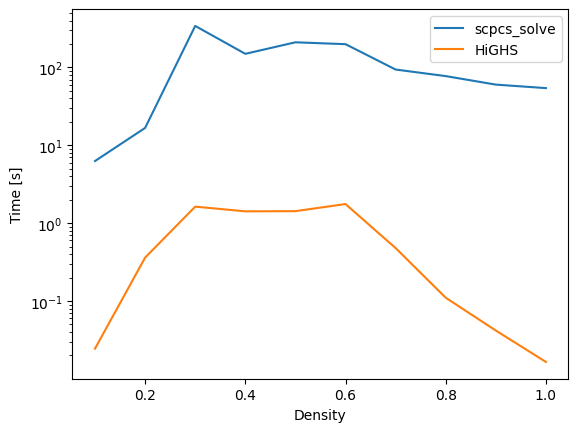
\includegraphics[width=0.6\columnwidth]{benchmark.png}
	\caption{Execution times}
	\label{fig:benchmark}
\end{figure}

The tests\footnote{Run on a laptop with an AMD Ryzen 4500U CPU and 8 GB of RAM} are carried out considering 10 instances with different average subset densities, with density for element $i$ defined as:
$$
d_i = \frac{|\{i \in S_j : S_j \in \mathcal{S}\}|}{|\mathcal{S}|}
$$
Subset densities are sampled from a (truncated) normal distribution with standard deviation equal to 0.01.

Figure \ref{fig:benchmark} reports execution times on instances with 40 elements and 40 subsets and varying density, with the penalty threshold set to 2. The proposed algorithm is around 100 times slower than HiGHS in all instances. An important aspect to consider is the tuning of the genetic algorithm, as population size and number of rounds should be tailored to the problem size; the trade-off is between a strong bound and a relatively small computational cost.
Time is spent almost completely in the subgradient optimization, as expected considering that the relaxation is a NP-hard problem. The greedy algorithm has a computational cost of $O(m \log m)$ in the worst case, considering at most $m$ extraction from the priority queue, where each extractions require a $O(\log m)$ cost for rearranging items in the underlying heap. The genetic algorithm complexity depends on the population size and the needed number of rounds; in this settings, the algorithm is executed once and took about 2 seconds for every instance.



\printbibliography

\end{document}